%Corps du document :
%\setlength{\parindent}{1cm}    

\section{Structures de données}
\subsection{Diagrammes UML détaillés}
\subsubsection{Structure XML}
\medskip
\begin {center}
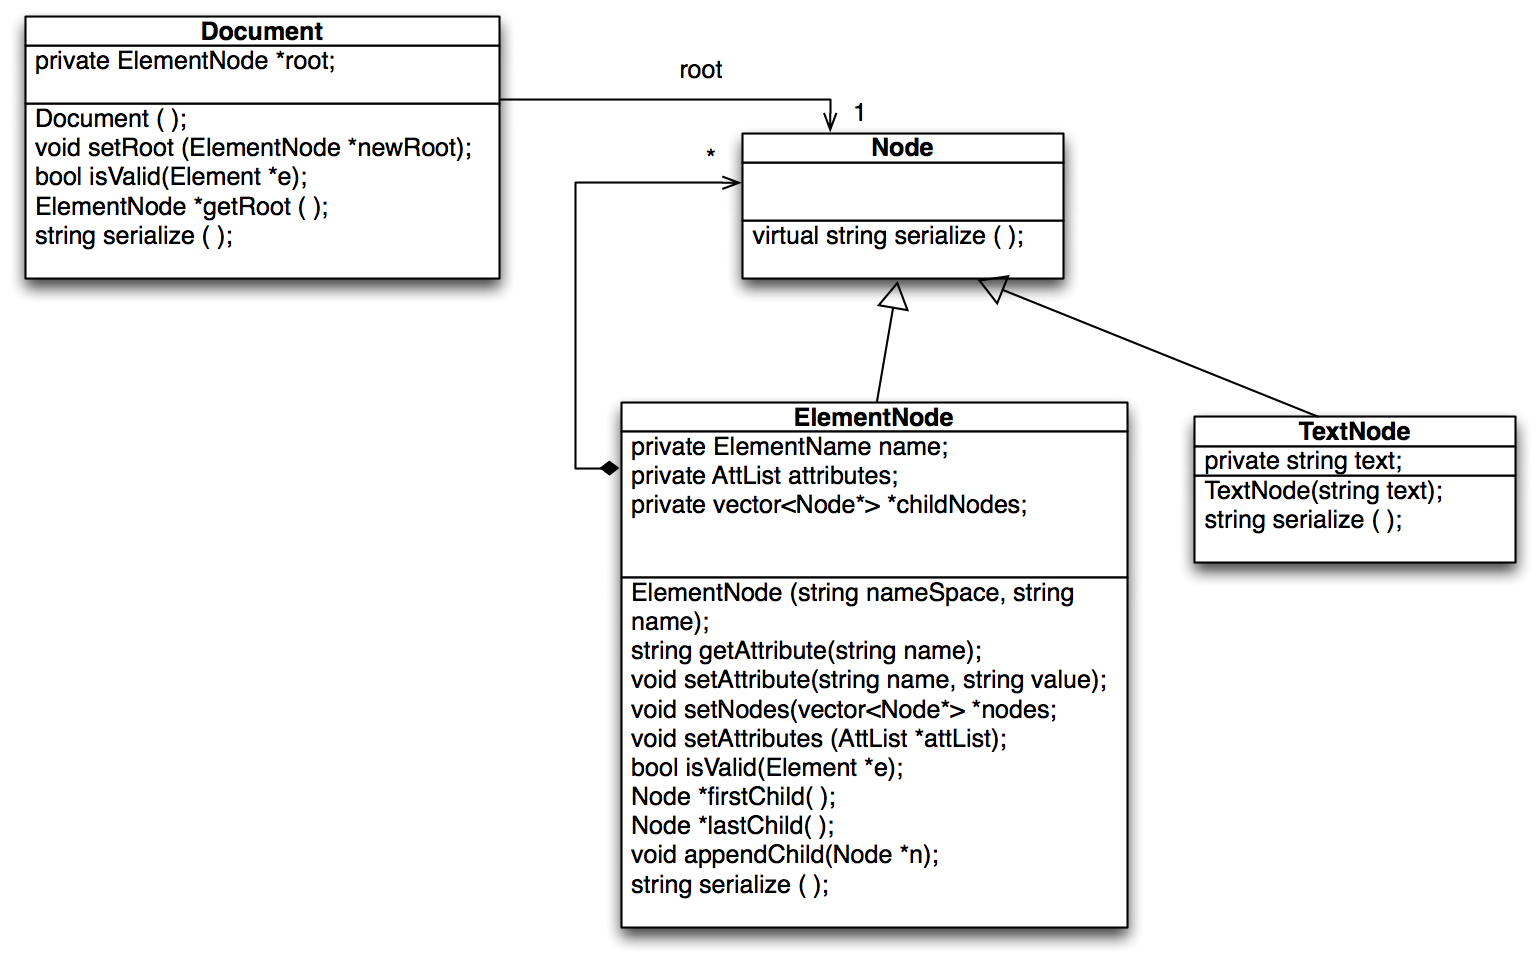
\includegraphics[width=\textwidth]{UMLXML.png}
\end {center}
\medskip
\subsubsection{Structure DTD}
\medskip
\begin {center}
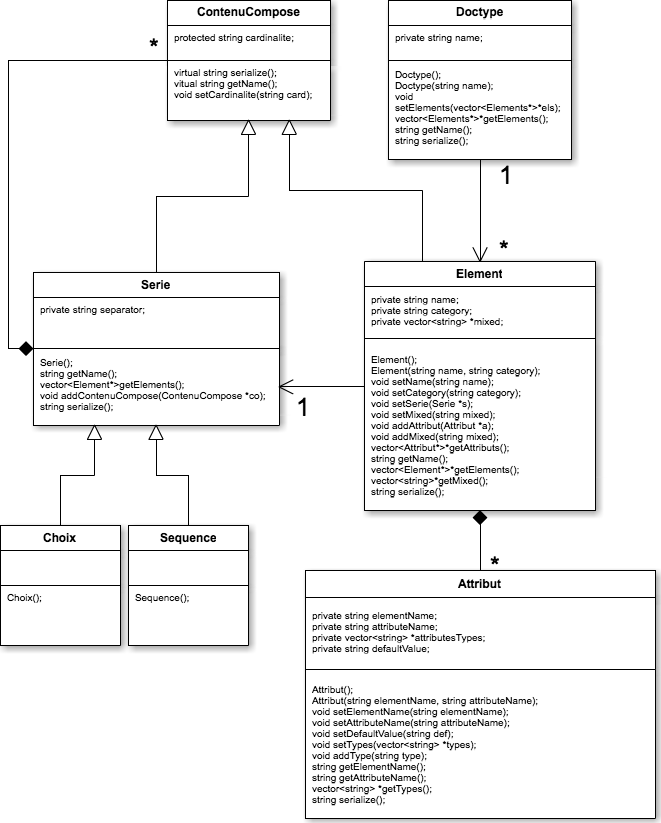
\includegraphics[width=\textwidth]{UMLDTD.png}
\end {center}
\medskip


\section{Algorithmes}

\subsection{Algorithmes de Validation}

\subsection{Algorithmes de Transformation}

\begin{algorithm}
\caption{TransformXML(documentXML,documentXSL)}
\begin{algorithmic}
\STATE $resultat \leftarrow new Document$
\FORALL{$template$}
\IF{$template de la raçine$}
\STATE $resultat.racine \leftarrow transformTemplate(templateRacine,elementNode de documentXML$
\ENDIF
\ENDFOR
\STATE $retour resultat$
end{algorithmic}
\end{algorithm}

\begin{algorithm}
\caption{TransformTemplate(nodeXML,template)}
\begin{algorithmic}
\STATE $result \leftarrow liste de node$
\IF{$template n'a pas le namespace xsl$}
\STATE $node \leftarrow new ElementNode(nom de template,attribut de template)$
\STATE $ajout de node dans result$
\ENDIF
\FORALL{$enfant de template$}
\IF{$enfant est un ElementNode$}
\IF{$namespace de l'enfant est xsl$}
\IF{$nom de l'enfant est apply-templates$}
\IF{$un template s'applique à un enfant de nodeXML$}
\STATE $result \leftarrow TransformTemplate(enfant de nodeXML,template à appliquer)$
\ENDIF
\ELSEIF{$nom de l'enfant est value-of$}
\STATE $result \leftarrow enfants de nodeXML$
\ENDIF
\ELSE
\STATE $result \leftarrow TransformTemplate(nodeXML,enfant du template)$
\ENDIF
\ELSE
\STATE $result \leftarrow enfant du template$
\ENDIF
\ENDFOR
\STATE $retour result$
end{algorithmic}
\end{algorithm}
